\documentclass[10pt,twocolumn]{article}

\usepackage{appendix}
\usepackage{graphicx}
\usepackage{pgfplots}
\usepackage{listings}
\lstset{
    frame=single,
    breaklines=true,
    numbers=left,
    xleftmargin=5.0ex
}

\title{High-Performance Linpack Optimization}

\author{
    Gurusiddesha Chandrasekhara\\
    Department of Informatics\\
    Technische Universit\"at M\"unchen\\
    guru.rvcs@gmail.com
  	\and
    Madhukar Sollepura Prabhu Shankar\\
    Department of Informatics\\
    Technische Universit\"at M\"unchen\\
    madhutime@gmail.com
    \and
    Madhura 	Kumaraswamy\\
    Department of Informatics\\
    Technische Universit\"at M\"unchen\\
    madhura.kswamy@gmail.com
    \and
    Lukas Grillmayer\\
    Department of Informatics\\
    Technische Universit\"at M\"unchen\\
    lukas.grillmayer@in.tum.de
}
\date{\today}

\begin{document}

\maketitle

\begin{abstract}
The purpose of this project is to automate the process of tuning parameters for the Linpack benchmark to obtain the optimal configuration. A Persicope plugin was created to perform this task. The plugin was then tested on consumer grade machines and built on the SuperMUC supercomputer. Results show the best scenario for manipulation of a set of parameters.
\end{abstract}

% ====================
\section{Introduction}
\label{sec:introduction}
% ====================
%DONE
Supercomputers embody the climax of high-performance computing (HPC) systems. They provide computation power for governments, industries, and researchers. Applications include the general areas of cryptanalysis, simulation, and modeling. With advancing technology the need for more computation power increases constantly in order to solve more complex problems. Demand-driven, the computation capabilities of supercomputers increase rapidly and many institutions compete for the most powerful system. The Top500 project biannually updates a list of the 500 best supercomputers based on the LINPACK benchmark, which measures the system's floating-point rate of execution. At the time of writing this paper, the best supercomputer is "Tianhe-2" at the National Super Computer Center in Guangzhou, China scoring 33.86 petaflops/s \cite{top500}.

LINPACK is a library which solves a dense system of linear equation in double precision on distributed-memory systems. The theoretical peak performance of a system is generally not achieved. For different problem sizes the actual performance is measured and maximized. Along with the problem size, the benchmark result is also influenced by other parameters which are discussed later.

\subsection{Project Description}
%DONE
The High Performance Linpack (HPL) benchmark has a configurable file called HPL.dat, which contains several parameters that may possibly impact the performance of a supercomputer. The goal of this project is to firstly, build HPL on the SuperMUC petascale system, and then, to identify which parameters impact the performance, with special regard to block sizes, type of process mapping (row-major or column-major) and type of swapping algorithm, and to determine how the problem size impacts scalability. Finally, to create a Periscope Tuning Framework (PTF) plugin that automates a new HPL.dat creation using "sed" (stream editor) and tunes the parameters in the SuperMUC system.

\subsection{Outline}
%DONE
In section \ref{sec:tools} tools are introduced which were used in the course of this project. Secondly, we discuss the tuning process and available benchmark parameters in detail before determining an initial configuration for a consumer grade laptop and SuperMUC. The implementation and functioning of the periscope plugin is described in section \ref{sec:implementation}. Next, the benchmark results are presented, highlighting the impact of the automated tuning process. In conclusion we summarize our findings and discuss topics for future work.

% ====================
\section{Tools}
\label{sec:tools}
% ====================

In this section, numerous tools are presented, which were used in the process of this project. This is list is non-exhaustive, so the scope was set to the most important programs.

\subsection{Periscope}
%long
Periscope is an online distributed performance analysis tool\cite{tibidabo} developed at the Technische Universit\"at M\"unchen that is used for dynamic tuning, which is a technique to automatically analyze performance issues of parallel MPI applications to evaluate single node performance\cite{tibidabo}. Periscope comprises an analysis agent network, consisting of three agents, namely, the master agent, communication agents and analysis agents, which search for performance problems in one or more experiments, called iterations and use a monitoring interface to configure the measurements. After the end of the search, the detected problems are communicated to the master agent through the communication agents and the results of the performance problem detection are displayed on a user-interface.


The Periscope Tuning Framework (PTF) was developed under the AutoTune project \cite{apsc} to combine and automate analysis and optimization of aspects such as energy consumption, inter-process communication and load balancing. PTF identifies tuning variants based on expert knowledge, evaluates the variants online and then, produces a report, which describes where and how to improve the code. PTF provides plugins for tuning high-level patterns for GPGPUs, HMPP codelets, MPI runtime, compiler flag selection and the energy consumption \cite{apsc}. 

\subsection{BLAS}
%short
Basic Linear Algebra Subprograms (BLAS) are a collection of routines which provide basic vector and matrix operations. It is efficient and portable, which makes it suitable for usage in high performance calculations. It is required by HPL \cite{blas}.

\subsection{ATLAS}
%short
Automatically Tuned Linear Algebra Software (ATLAS) provides a complete BLAS API for C and Fortran77. For all operations it optimizes performance for a specific machine, allowing it to execute faster than plain BLAS. Since HPL requires BLAS it can be substituted by ATLAS \cite{atlas}.


\subsection{Open MPI}
%long
OpenMPI is an open source implementation of MPI (Message Passing Interface), a message passing library specification commonly used in the HPC community. Maintained by numerous academic, research, and industry partners this platform independent interface became the industry-standard for parallel programs in the last decade and has reached version 3.0 in September 2012. When the MPI project started in 1993 the objective was to unify a variety of libraries and form a standardized solution. As it is designed for portability, efficiency, and flexibility, MPI runs on virtually any distributed memory, shared memory, and hybrid systems. Among others, the MPI interface has been implemented for C, C++, Fortran, and Python \cite{mpitut, ompi}.


MPI uses Virtual Topology, Communicator and Group objects to form a communication domain for a set of processes. A Communicator assigns a unique identifier to each process, which can be used  to specify source and destination of messages. By default the program aborts if MPI encounters any error \cite{ompi}.

\subsection{High-Performance Linpack}
LINPACK addresses scalability in distributed memory systems by providing additional testing rules and environment through the Highly-Parallel LINPACK (HPL) NxN benchmark, which is used for measuring supercomputer performance in the Top500 list. HPL is a portable implementation of the HPL NxN benchmark, and generates and solves a random dense linear system of equations using Gaussian Elimination with partial pivoting and double precision floating point arithmetic. The HPL package is written in C and requires the implementation of either the BLAS library, which can be automatically generated by the ATLAS tool, or the Vector Signal Image Processing Library (VSIPL). The HPL package provides testing rules to obtain the accuracy of the obtained solution, and timing rules to obtain the computation time to determine the best performance scenario.  

The computational steps performed by HPL to obtain the benchmark rating are :

\begin{lstlisting}
/* Generate and partition matrix data among MPI computing nodes. */
/* ... */

/* All the nodes start at the same time. */
MPI_Barrier(...);

/* Start wall-clock timer. */
HPL_ptimer(...);

/* Solve system of equations. */
HPL_pdgesv(...);

/* Stop wall-clock timer. */
HPL_ptimer(...);

/* Obtain the maximum wall-clock time. */
MPI_Reduce(...);

/* Gather statistics about perofrmance rate (based on the maximum wall-clock time) and accuracy of the solution. */
/* ... */

\end{lstlisting}


\subsubsection{Scalabilty}
Scalability is an important aspect that must be considered while running problems on thousands of nodes. Strong scaling is the process of fixing a workload or the problem size and increasing the number of processors so that a program scales linearly when the speedup increases with the number of processing elements used. With respect to the total energy consumption, embarrassingly parallel codes achieve better energy efficiency with increasing system size[1]. Weak scaling is the process of increasing both the workload or the problem size and the number of processors so that the program scales linearly when the run-time stays constant while increasing the workload or problem size proportionally to the number of processors. HPL is a good weakly scalable application and gets more efficient with increasing memory \cite{tibidabo}.


\subsection{Installation Script}
%DONE
We created a installation script (see appendix \ref{sec:appendix_installationScript}) which automates the installation process of Periscope and HPL with all dependents. It was created for deployment on a clean installation of Ubuntu 14.04 LTS 64bit Desktop using VirtualBox. We suggest a hard disk size of 16GB or larger. The installation process also depends on the system properties, the installation script can serve as useful guideline.


% ====================
\section{Tuning}
\label{sec:tuning}
% ====================

As discussed before HPL needs a set of parameters to derive a scenario for benchmarking. This is done via the HPL.dat file, which lists all available options. If multiple values are provided for individual parameters, HPL will execute all possible combinations in a separate scenario. In the following, parameters relevant for benchmarking are presented \cite{HPLtuning, HPLexplained}.

\subsection{Parameters}
\label{sec:tuning_parameters}

\begin{itemize}

\item Problem size (N): The problem should be as large as possible, whereas N denotes the size of the coefficient matrix. If the problem size exceeds the available memory, performance will decrease due to swapping. It is suggested to initially use about 80\% of available memory.
\begin{center}
$ N = sqrt ( ( \#nodes * \#memoryPerNode * 0.8 ) / sizeOf(double) )$
\end{center}

\item Block size (NB): It is used for data distribution and computational granularity. Small values are desired as data distribution and load balancing improves. If chosen too small, the message overhead will increase and the available cache hierarchy might not be used properly. A value between 32 and 256 is suggested for modern systems.

\item Process grid size (PxQ): The number of process rows (P) and columns (Q) depends on the number of available nodes and the physical network connection. It defines the number of nodes onto which HPL data should be distributed and executed, the process grid. Q must be slightly larger or equal to P. For simple Ethernet networks P should be very small since network scaling is limited. $P*Q$ must be equal to the number of nodes in the system. If surpassed, additional nodes will not be utilized. The suggested range is:
\begin{center}
$P \leq Q \leq 3*P$	
\end{center}

\item Residual threshold: The residuals of the main algorithm will be compared to this value. The threshold is a real number of magnitude 1, whereas for negative values this threshold will not be checked. A suggested value is $16.0$.

\item Recursive factorization method (RFACT): Panel factorization is a matrix-matrix operation, which divides a large matrix into several submatrices. This is also known as LU decomposition. The left-looking and right-looking variants of this algorithm comply to the Doolittle method, dividing the matrix into lower and upper triangular unit matrices. The Crout variant is similar, but the returned lower matrix is not a unit matrix.

\item Panels in recursion (NDIV): During each iteration of panel factorization the current matrix is divided into NDIV submatrices.

\item Recursion stopping criteria (NBMIN): The panel factorization recursion stops when the matrix is is composed of NBMIN columns or less.

\item Panel factorization method (PFACT): After the factorization recursion stops, the algorithm continues with LU decomposition on a matrix-vector basis using a left-looking, Crout, or right-looking approach defined by RFACT.

\item Lookahead depth (DEPTH): The lookahead depth defines the number of next panels which should be factorized immediately after being updated. For large problem sizes a value of 1 is suggested.

\item Panel broadcasting method (BCAST): After panel factorization is complete, the resulting values are sent to other process columns using messages. Using different approaches leads to changes in execution time and throughput. There are multiple broadcast algorithms available:
\begin{itemize}
\item Increased-ring: Every process has to send a message the next process consequently.
\item Increased-ring (modified): Process 0 sends a message to process 1 and 2 each. 
\item Increasing-2-ring: Processes are split into two groups, whereas process 0 sends a message to the second group and acts as the first element of the first group.
\item Increasing-2-ring (modified): The modification to increasing-2-ring is to additionally apply the increasing-ring algorithm to the first group.
\item Long (bandwidth-reducing): The message is divided into Q equal pieces to be distributed to Q different processes in a synchronized fashion. The submessages are then exchanged between sets of two processes until every process received all parts of the original message.
\item Long (bandwidth-reducing modified): The modification to long (bandwidth reducing) is to additionally apply the increasing-ring algorithm.
\end{itemize}

The best method depends on the problem size and hardware performance. If the platform nodes are expected to outperform the network, "Long (bandwidth reducing)" (Lng) or "Long (bandwith reducing modified)" (LnM) can be recommended.

\item Process mapping(PMAP): This parameter specifies how the MPI processes are mapped to the nodes. It is recommended to use row-major mapping for systems with multi-processor computer nodes.

\item Swap algorithm (SWAP): This parameter specifies the swapping algorithm used during all tests. Available algorithms are based on binary-exchange (bin) and spread-roll (long). For mix, the binary-exchange will be used for a number of columns less than the swapping threshold before switching to spread-roll. The swapping threshold is only used for mix. For bin and long, the equilibrium phase can be enabled / disabled.

\item Storage of panel triangle (L1, U): These parameters specify whether the lower (L1) and upper (U) triangle matrix should be stored in no-transposed or transposed form.

\item Memory alignment: This parameters specifies the memory alignment HPL uses to allocate memory. The value is measured in double.
\end{itemize}

For the purpose of this project following parameters were considered for optimization:
\begin{itemize}
\item Problem size (N)
\item Block size (NB)
\item Process grid size (PxQ)
\item Process mapping (PMAP)
%\item Swap algorithm (SWAP)
%\item Panel broadcasting method (BCAST)
\end{itemize}

Appendix \ref{sec:appendixHPLdatLaptop} shows the optimal configuration for a Lenovo G510 laptop.



% ====================
\section{Implementation}
\label{sec:implementation}
% ====================

A Periscope plugin must implement the "Tuning Plugin Interface (TPI)". This interface requires developers to follow the generic flow displayed in figure \ref{fig:flow}. As some steps are optional only the steps relevant to the implementation of this project's plugin are discussed in this section \cite{flow}.

\begin{figure}[h]
	\centering
	\includegraphics[scale=0.5]{ptf_flow}
	\caption{PTF plugin flow \cite{flow}}
	\label{fig:flow}
\end{figure}

\begin{itemize}

\item Initialize: First set the context and pool\_set references, passed by the runtime system to the plugin, define the search algorithm and set the tuning parameters in the following way.
\end{itemize}
\begin{lstlisting}
//Problem Size ranging from 6000 to 10000 [Increasing in steps of 1000]
TuningParameter *inputSizeTP = new TuningParameter();
inputSizeTP->setId(0);
inputSizeTP->setName("PROBLEMSIZE");
inputSizeTP->setRange(6000, 10000, 1000); // (start, max, step)
tuningParameters.push_back(inputSizeTP);
\end{lstlisting}

\begin{itemize}

\item Start Tuning: Create instances of Variant space and Search space. Add each tuning parameter to variant space and set variant space to search space. Finally add search space to search algorithm.

\item Analysis Required: Perform analysis of the application in this step. If no analysis is not required, then return false. 

\item Create Scenario: Create the scenario for the application and place it in create scenario pool.

\item Prepare scenario: Retrieve the scenario from create scenario pool. Extract the integral value from it. Use these values to update the application specific file. Example: For HPL application, we are updating HPL.dat file with necessary value using 'sed' command. It's as shown below. Later push the scenario to prepared scenario pool.
\end{itemize}
\begin{lstlisting}
const Variant* v = scenario->getTuningSpecifications()->front()->getVariant();
map<TuningParameter*,int> tpValues = v->getValue();
long problemSize = tpValues[tuningParameters[0]];
long blockSize = tpValues[tuningParameters[1]];
long pMapping = tpValues[tuningParameters[2]];
long qMapping = tpValues[tuningParameters[3]];
long procMapping = tpValues[tuningParameters[4]];

sprintf(cmnd,"sed -e '6s/.*/%ld/' -e '8s/.*/%ld/' -e '11s/.*/%ld/' -e '12s/.*/%ld/' -e '9s/.*/%ld/' -e '3s/.*/HPL%d.out/' <HPL.dat.sed >HPL.dat ", problemSize, blockSize, pMapping, qMapping, procMapping, hplcounter++);
\end{lstlisting}

\begin{itemize}


\item Define experiment: Get scenario from prepared scenario pool and push it to experiment scenario pool. After this operation, the runtime system performs the experiment to acquire the specified properties. In our case it acquired execution time.

\item Restart Required: Specify restart is required for next experiment by returning value as true, otherwise false.

\item Search Finished: Return true if search is finished, otherwise false.

\item Finish Tuning: The post processing operation are performed here, before entering to next tuning iteration.

\item Tuning finished: Return true, if plugin has finished tuning process, otherwise false.

\item Get Advice: Provide resulting information to the user in a file. In our case, we extracted the Gflops value from a temporary result file using a user defined function 'extract'. Following command was used to extract time and Gflops information from output file.
\end{itemize}

\begin{lstlisting}
sprintf(cmnd,"awk '/WR/{print %d \"\\t\"$6 \"\\t\"$7}' HPL%d.out >> TimeAndGflops", (hplcounter - 1),(hplcounter - 1)); 
\end{lstlisting}

\begin{itemize}

\item Finalize: All created objects are freed in this method.

\end{itemize}


% ====================
\section{Evaluation}
\label{sec:evaluation}
% ====================
The plugin was executed on a Lenovo G510 laptop (Intel i7-4700MQ $@$ 2.4 GHz, 8.0GB PC3-12800 DDR3 SDRAM $@$ 1.6Ghz) conducting 270 experiments with various parameter configurations. It was determined that the configuration shown in appendix \ref{sec:appendixHPLdatLaptop} yielded the best results, with an actual performance of 30.13 Gflops. The plugin correctly pointed to scenario 230 as optimal solution for the executed experiments. The following subsections show the results of this benchmark in detail.

\subsection{Problem Size}
The problem size for a system should be as large as possible (see section \ref{sec:tuning_parameters}). Figure \ref{fig:N} shows that a problem size of 10,000 yielded the best results. It depicts the impact of the problem size ordered by performance:

\begin{figure}[h]
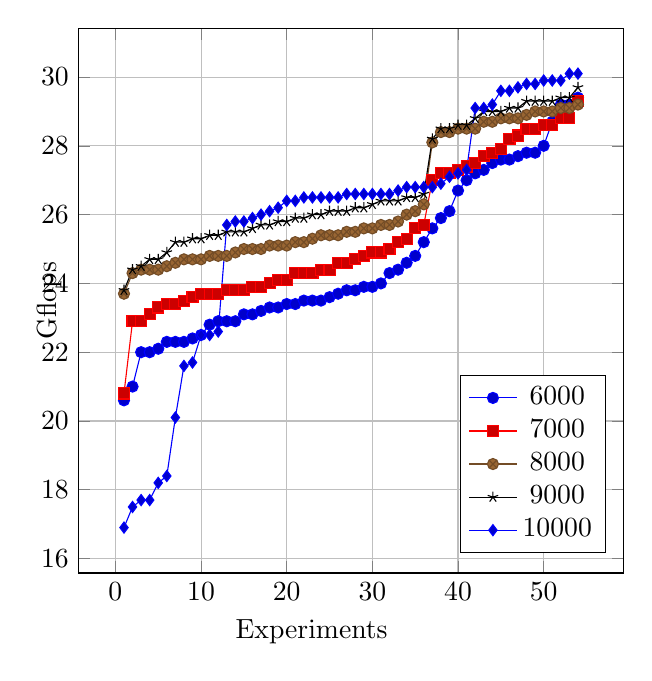
\begin{tikzpicture} 
	\begin{axis}[ 
        ylabel={Gflops},ylabel style={yshift=-0.5cm},
        xlabel={Experiments},xlabel style={xshift=-0.5cm},
		height=8.5cm, 
		width=8.5cm, 
		grid=major, 
		legend style={at={(0.7,0.2)},anchor=west},
	] 
	
	\addplot coordinates { 
	(1,2.06E+001)(2,2.10E+001)(3,2.20E+001)(4,2.20E+001)(5,2.21E+001)(6,2.23E+001)(7,2.23E+001)(8,2.23E+001)(9,2.24E+001)(10,2.25E+001)(11,2.28E+001)(12,2.29E+001)(13,2.29E+001)(14,2.29E+001)(15,2.31E+001)(16,2.31E+001)(17,2.32E+001)(18,2.33E+001)(19,2.33E+001)(20,2.34E+001)(21,2.34E+001)(22,2.35E+001)(23,2.35E+001)(24,2.35E+001)(25,2.36E+001)(26,2.37E+001)(27,2.38E+001)(28,2.38E+001)(29,2.39E+001)(30,2.39E+001)(31,2.40E+001)(32,2.43E+001)(33,2.44E+001)(34,2.46E+001)(35,2.48E+001)(36,2.52E+001)(37,2.56E+001)(38,2.59E+001)(39,2.61E+001)(40,2.67E+001)(41,2.70E+001)(42,2.72E+001)(43,2.73E+001)(44,2.75E+001)(45,2.76E+001)(46,2.76E+001)(47,2.77E+001)(48,2.78E+001)(49,2.78E+001)(50,2.80E+001)(51,2.87E+001)(52,2.92E+001)(53,2.92E+001)(54,2.94E+001)
	}; 
	\addlegendentry{6000} 
	
	\addplot coordinates { 
	(1,2.08E+001)(2,2.29E+001)(3,2.29E+001)(4,2.31E+001)(5,2.33E+001)(6,2.34E+001)(7,2.34E+001)(8,2.35E+001)(9,2.36E+001)(10,2.37E+001)(11,2.37E+001)(12,2.37E+001)(13,2.38E+001)(14,2.38E+001)(15,2.38E+001)(16,2.39E+001)(17,2.39E+001)(18,2.40E+001)(19,2.41E+001)(20,2.41E+001)(21,2.43E+001)(22,2.43E+001)(23,2.43E+001)(24,2.44E+001)(25,2.44E+001)(26,2.46E+001)(27,2.46E+001)(28,2.47E+001)(29,2.48E+001)(30,2.49E+001)(31,2.49E+001)(32,2.50E+001)(33,2.52E+001)(34,2.53E+001)(35,2.56E+001)(36,2.57E+001)(37,2.70E+001)(38,2.72E+001)(39,2.72E+001)(40,2.73E+001)(41,2.74E+001)(42,2.75E+001)(43,2.77E+001)(44,2.78E+001)(45,2.79E+001)(46,2.82E+001)(47,2.83E+001)(48,2.85E+001)(49,2.85E+001)(50,2.86E+001)(51,2.86E+001)(52,2.88E+001)(53,2.88E+001)(54,2.93E+001)
	}; 
	\addlegendentry{7000} 
	
	\addplot coordinates { 
	(1,2.37E+001)(2,2.43E+001)(3,2.44E+001)(4,2.44E+001)(5,2.44E+001)(6,2.45E+001)(7,2.46E+001)(8,2.47E+001)(9,2.47E+001)(10,2.47E+001)(11,2.48E+001)(12,2.48E+001)(13,2.48E+001)(14,2.49E+001)(15,2.50E+001)(16,2.50E+001)(17,2.50E+001)(18,2.51E+001)(19,2.51E+001)(20,2.51E+001)(21,2.52E+001)(22,2.52E+001)(23,2.53E+001)(24,2.54E+001)(25,2.54E+001)(26,2.54E+001)(27,2.55E+001)(28,2.55E+001)(29,2.56E+001)(30,2.56E+001)(31,2.57E+001)(32,2.57E+001)(33,2.58E+001)(34,2.60E+001)(35,2.61E+001)(36,2.63E+001)(37,2.81E+001)(38,2.84E+001)(39,2.84E+001)(40,2.85E+001)(41,2.85E+001)(42,2.85E+001)(43,2.87E+001)(44,2.87E+001)(45,2.88E+001)(46,2.88E+001)(47,2.88E+001)(48,2.89E+001)(49,2.90E+001)(50,2.90E+001)(51,2.90E+001)(52,2.91E+001)(53,2.91E+001)(54,2.92E+001)
	}; 
	\addlegendentry{8000} 
	
	\addplot coordinates { 
	(1,2.38E+001)(2,2.44E+001)(3,2.45E+001)(4,2.47E+001)(5,2.47E+001)(6,2.49E+001)(7,2.52E+001)(8,2.52E+001)(9,2.53E+001)(10,2.53E+001)(11,2.54E+001)(12,2.54E+001)(13,2.55E+001)(14,2.55E+001)(15,2.55E+001)(16,2.56E+001)(17,2.57E+001)(18,2.57E+001)(19,2.58E+001)(20,2.58E+001)(21,2.59E+001)(22,2.59E+001)(23,2.60E+001)(24,2.60E+001)(25,2.61E+001)(26,2.61E+001)(27,2.61E+001)(28,2.62E+001)(29,2.62E+001)(30,2.63E+001)(31,2.64E+001)(32,2.64E+001)(33,2.64E+001)(34,2.65E+001)(35,2.65E+001)(36,2.66E+001)(37,2.82E+001)(38,2.85E+001)(39,2.85E+001)(40,2.86E+001)(41,2.86E+001)(42,2.88E+001)(43,2.90E+001)(44,2.90E+001)(45,2.90E+001)(46,2.91E+001)(47,2.91E+001)(48,2.93E+001)(49,2.93E+001)(50,2.93E+001)(51,2.93E+001)(52,2.94E+001)(53,2.94E+001)(54,2.97E+001)
	}; 
	\addlegendentry{9000} 
	
	\addplot coordinates { 
	(1,1.69E+001)(2,1.75E+001)(3,1.77E+001)(4,1.77E+001)(5,1.82E+001)(6,1.84E+001)(7,2.01E+001)(8,2.16E+001)(9,2.17E+001)(10,2.25E+001)(11,2.25E+001)(12,2.26E+001)(13,2.57E+001)(14,2.58E+001)(15,2.58E+001)(16,2.59E+001)(17,2.60E+001)(18,2.61E+001)(19,2.62E+001)(20,2.64E+001)(21,2.64E+001)(22,2.65E+001)(23,2.65E+001)(24,2.65E+001)(25,2.65E+001)(26,2.65E+001)(27,2.66E+001)(28,2.66E+001)(29,2.66E+001)(30,2.66E+001)(31,2.66E+001)(32,2.66E+001)(33,2.67E+001)(34,2.68E+001)(35,2.68E+001)(36,2.68E+001)(37,2.68E+001)(38,2.69E+001)(39,2.71E+001)(40,2.72E+001)(41,2.73E+001)(42,2.91E+001)(43,2.91E+001)(44,2.92E+001)(45,2.96E+001)(46,2.96E+001)(47,2.97E+001)(48,2.98E+001)(49,2.98E+001)(50,2.99E+001)(51,2.99E+001)(52,2.99E+001)(53,3.01E+001)(54,3.01E+001)
	}; 
	\addlegendentry{10000} 
	\end{axis} 
\end{tikzpicture}
	\caption{Performance impact of problem size}
	\label{fig:N}
\end{figure}


\subsection{Block Size}
Figure \ref{fig:NB} indicates that block size has only a minor impact on performance readings. The best performance was reached with a block size of 160.

\begin{figure}[h]
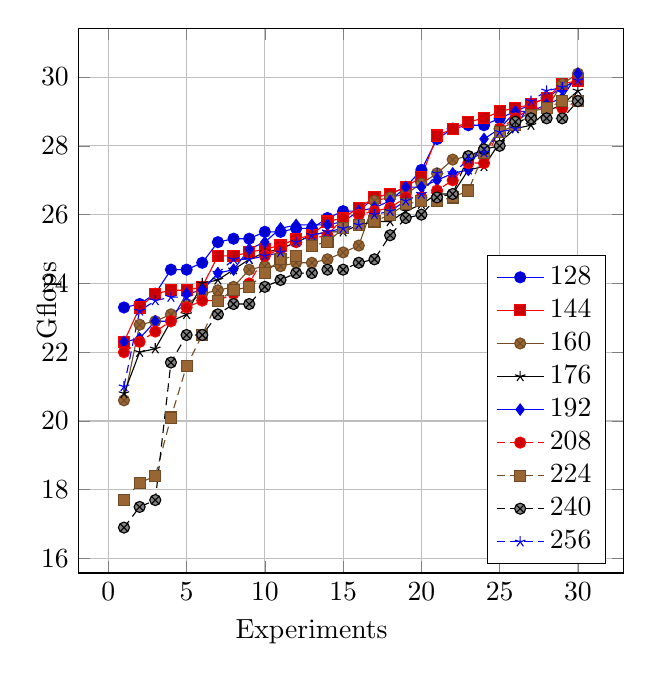
\begin{tikzpicture} 
	\begin{axis}[ 
        ylabel={Gflops},ylabel style={yshift=-0.5cm},
        xlabel={Experiments},xlabel style={xshift=-0.5cm},
		height=8.5cm, 
		width=8.5cm, 
		grid=major, 
		legend style={at={(0.75,0.3)},anchor=west},
	] 
	
	\addplot coordinates { 
	(1,2.33E+001)(2,2.34E+001)(3,2.37E+001)(4,2.44E+001)(5,2.44E+001)(6,2.46E+001)(7,2.52E+001)(8,2.53E+001)(9,2.53E+001)(10,2.55E+001)(11,2.55E+001)(12,2.56E+001)(13,2.56E+001)(14,2.59E+001)(15,2.61E+001)(16,2.61E+001)(17,2.65E+001)(18,2.66E+001)(19,2.68E+001)(20,2.73E+001)(21,2.82E+001)(22,2.85E+001)(23,2.86E+001)(24,2.86E+001)(25,2.88E+001)(26,2.90E+001)(27,2.92E+001)(28,2.94E+001)(29,2.97E+001)(30,2.99E+001)
	}; 
	\addlegendentry{128} 
	
	\addplot coordinates { 
	(1,2.23E+001)(2,2.33E+001)(3,2.37E+001)(4,2.38E+001)(5,2.38E+001)(6,2.39E+001)(7,2.48E+001)(8,2.48E+001)(9,2.49E+001)(10,2.50E+001)(11,2.51E+001)(12,2.53E+001)(13,2.54E+001)(14,2.58E+001)(15,2.59E+001)(16,2.62E+001)(17,2.65E+001)(18,2.66E+001)(19,2.68E+001)(20,2.71E+001)(21,2.83E+001)(22,2.85E+001)(23,2.87E+001)(24,2.88E+001)(25,2.90E+001)(26,2.91E+001)(27,2.92E+001)(28,2.94E+001)(29,2.98E+001)(30,2.99E+001)
	}; 
	\addlegendentry{144} 
	
	\addplot coordinates { 
	(1,2.06E+001)(2,2.28E+001)(3,2.29E+001)(4,2.31E+001)(5,2.34E+001)(6,2.37E+001)(7,2.38E+001)(8,2.39E+001)(9,2.44E+001)(10,2.45E+001)(11,2.45E+001)(12,2.46E+001)(13,2.46E+001)(14,2.47E+001)(15,2.49E+001)(16,2.51E+001)(17,2.64E+001)(18,2.65E+001)(19,2.66E+001)(20,2.69E+001)(21,2.72E+001)(22,2.76E+001)(23,2.77E+001)(24,2.78E+001)(25,2.85E+001)(26,2.87E+001)(27,2.90E+001)(28,2.91E+001)(29,2.98E+001)(30,3.01E+001)
	}; 
	\addlegendentry{160} 
	
	\addplot coordinates { 
	(1,2.08E+001)(2,2.20E+001)(3,2.21E+001)(4,2.29E+001)(5,2.31E+001)(6,2.40E+001)(7,2.41E+001)(8,2.44E+001)(9,2.47E+001)(10,2.49E+001)(11,2.50E+001)(12,2.52E+001)(13,2.54E+001)(14,2.55E+001)(15,2.55E+001)(16,2.57E+001)(17,2.58E+001)(18,2.58E+001)(19,2.61E+001)(20,2.63E+001)(21,2.66E+001)(22,2.66E+001)(23,2.73E+001)(24,2.74E+001)(25,2.81E+001)(26,2.85E+001)(27,2.86E+001)(28,2.90E+001)(29,2.92E+001)(30,2.96E+001)
	}; 
	\addlegendentry{176} 
	
	\addplot coordinates { 
	(1,2.23E+001)(2,2.24E+001)(3,2.29E+001)(4,2.29E+001)(5,2.37E+001)(6,2.38E+001)(7,2.43E+001)(8,2.44E+001)(9,2.50E+001)(10,2.52E+001)(11,2.56E+001)(12,2.57E+001)(13,2.57E+001)(14,2.57E+001)(15,2.58E+001)(16,2.61E+001)(17,2.62E+001)(18,2.64E+001)(19,2.68E+001)(20,2.68E+001)(21,2.70E+001)(22,2.72E+001)(23,2.73E+001)(24,2.82E+001)(25,2.85E+001)(26,2.90E+001)(27,2.90E+001)(28,2.92E+001)(29,2.94E+001)(30,3.01E+001)
	}; 
	\addlegendentry{192}
	
	\addplot coordinates { 
	(1,2.20E+001)(2,2.23E+001)(3,2.26E+001)(4,2.29E+001)(5,2.33E+001)(6,2.35E+001)(7,2.35E+001)(8,2.37E+001)(9,2.40E+001)(10,2.48E+001)(11,2.50E+001)(12,2.52E+001)(13,2.53E+001)(14,2.54E+001)(15,2.59E+001)(16,2.60E+001)(17,2.61E+001)(18,2.62E+001)(19,2.65E+001)(20,2.65E+001)(21,2.67E+001)(22,2.70E+001)(23,2.75E+001)(24,2.75E+001)(25,2.85E+001)(26,2.88E+001)(27,2.91E+001)(28,2.91E+001)(29,2.91E+001)(30,2.93E+001)	
	}; 
	\addlegendentry{208}
	
	\addplot coordinates { 
	(1,1.77E+001)(2,1.82E+001)(3,1.84E+001)(4,2.01E+001)(5,2.16E+001)(6,2.25E+001)(7,2.35E+001)(8,2.38E+001)(9,2.39E+001)(10,2.43E+001)(11,2.47E+001)(12,2.48E+001)(13,2.51E+001)(14,2.52E+001)(15,2.56E+001)(16,2.57E+001)(17,2.58E+001)(18,2.60E+001)(19,2.63E+001)(20,2.64E+001)(21,2.64E+001)(22,2.65E+001)(23,2.67E+001)(24,2.78E+001)(25,2.84E+001)(26,2.86E+001)(27,2.89E+001)(28,2.91E+001)(29,2.93E+001)(30,2.93E+001)
	}; 
	\addlegendentry{224}
	
	\addplot coordinates { 
	(1,1.69E+001)(2,1.75E+001)(3,1.77E+001)(4,2.17E+001)(5,2.25E+001)(6,2.25E+001)(7,2.31E+001)(8,2.34E+001)(9,2.34E+001)(10,2.39E+001)(11,2.41E+001)(12,2.43E+001)(13,2.43E+001)(14,2.44E+001)(15,2.44E+001)(16,2.46E+001)(17,2.47E+001)(18,2.54E+001)(19,2.59E+001)(20,2.60E+001)(21,2.65E+001)(22,2.66E+001)(23,2.77E+001)(24,2.79E+001)(25,2.80E+001)(26,2.87E+001)(27,2.88E+001)(28,2.88E+001)(29,2.88E+001)(30,2.93E+001)
	}; 
	\addlegendentry{240}
	
	\addplot coordinates { 
	(1,2.10E+001)(2,2.32E+001)(3,2.35E+001)(4,2.36E+001)(5,2.36E+001)(6,2.38E+001)(7,2.43E+001)(8,2.47E+001)(9,2.47E+001)(10,2.48E+001)(11,2.49E+001)(12,2.52E+001)(13,2.54E+001)(14,2.55E+001)(15,2.56E+001)(16,2.57E+001)(17,2.60E+001)(18,2.61E+001)(19,2.64E+001)(20,2.66E+001)(21,2.72E+001)(22,2.72E+001)(23,2.76E+001)(24,2.78E+001)(25,2.84E+001)(26,2.85E+001)(27,2.93E+001)(28,2.96E+001)(29,2.97E+001)(30,2.99E+001)
	}; 
	\addlegendentry{256}
	
	\end{axis} 
\end{tikzpicture}
	\caption{Performance impact of block size}
	\label{fig:NB}
\end{figure}


\subsection{Process Grid (P x Q)}
The process grid size should be equal to the number of cores per node (see section \ref{sec:tuning_parameters}). A common misconception is the assumption that the cores presented in monitoring programs like Microsoft Windows Task Manager are real cores. By utilizing Hyperthreading, a single hardware core can be split in two threads. As a result, the performance measurements were significantly lower on experiments which utilized more than the physically available four cores. Figure \ref{fig:PQ} indicates that a process grid size of 2x2 yields the best results.

\begin{figure}[h]
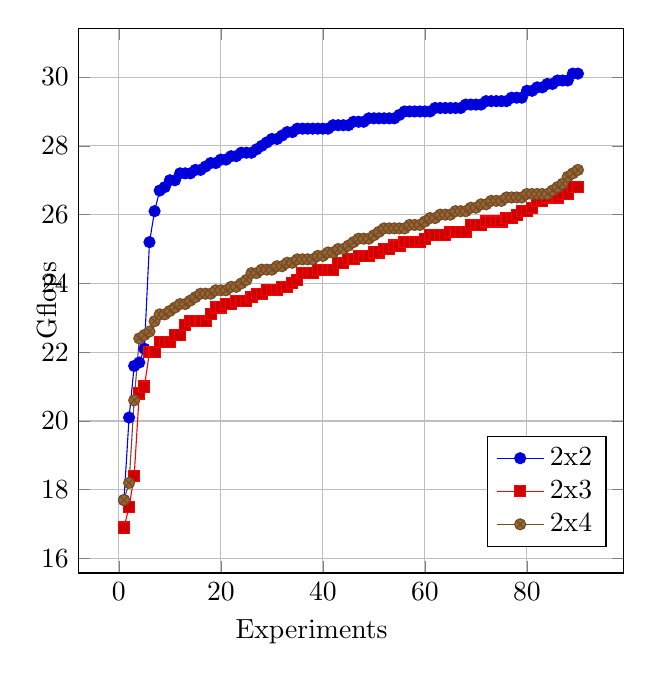
\begin{tikzpicture} 
	\begin{axis}[ 
        ylabel={Gflops},ylabel style={yshift=-0.5cm},
        xlabel={Experiments},xlabel style={xshift=-0.5cm},
		height=8.5cm, 
		width=8.5cm, 
		grid=major, 
		legend style={at={(0.75,0.15)},anchor=west},
	] 
	
	\addplot coordinates { 
	(1,1.77E+001)(2,2.01E+001)(3,2.16E+001)(4,2.17E+001)(5,2.21E+001)(6,2.52E+001)(7,2.61E+001)(8,2.67E+001)(9,2.68E+001)(10,2.70E+001)(11,2.70E+001)(12,2.72E+001)(13,2.72E+001)(14,2.72E+001)(15,2.73E+001)(16,2.73E+001)(17,2.74E+001)(18,2.75E+001)(19,2.75E+001)(20,2.76E+001)(21,2.76E+001)(22,2.77E+001)(23,2.77E+001)(24,2.78E+001)(25,2.78E+001)(26,2.78E+001)(27,2.79E+001)(28,2.80E+001)(29,2.81E+001)(30,2.82E+001)(31,2.82E+001)(32,2.83E+001)(33,2.84E+001)(34,2.84E+001)(35,2.85E+001)(36,2.85E+001)(37,2.85E+001)(38,2.85E+001)(39,2.85E+001)(40,2.85E+001)(41,2.85E+001)(42,2.86E+001)(43,2.86E+001)(44,2.86E+001)(45,2.86E+001)(46,2.87E+001)(47,2.87E+001)(48,2.87E+001)(49,2.88E+001)(50,2.88E+001)(51,2.88E+001)(52,2.88E+001)(53,2.88E+001)(54,2.88E+001)(55,2.89E+001)(56,2.90E+001)(57,2.90E+001)(58,2.90E+001)(59,2.90E+001)(60,2.90E+001)(61,2.90E+001)(62,2.91E+001)(63,2.91E+001)(64,2.91E+001)(65,2.91E+001)(66,2.91E+001)(67,2.91E+001)(68,2.92E+001)(69,2.92E+001)(70,2.92E+001)(71,2.92E+001)(72,2.93E+001)(73,2.93E+001)(74,2.93E+001)(75,2.93E+001)(76,2.93E+001)(77,2.94E+001)(78,2.94E+001)(79,2.94E+001)(80,2.96E+001)(81,2.96E+001)(82,2.97E+001)(83,2.97E+001)(84,2.98E+001)(85,2.98E+001)(86,2.99E+001)(87,2.99E+001)(88,2.99E+001)(89,3.01E+001)(90,3.01E+001)
	}; 
	\addlegendentry{2x2} 
	
	\addplot coordinates { 
	(1,1.69E+001)(2,1.75E+001)(3,1.84E+001)(4,2.08E+001)(5,2.10E+001)(6,2.20E+001)(7,2.20E+001)(8,2.23E+001)(9,2.23E+001)(10,2.23E+001)(11,2.25E+001)(12,2.25E+001)(13,2.28E+001)(14,2.29E+001)(15,2.29E+001)(16,2.29E+001)(17,2.29E+001)(18,2.31E+001)(19,2.33E+001)(20,2.33E+001)(21,2.34E+001)(22,2.34E+001)(23,2.35E+001)(24,2.35E+001)(25,2.35E+001)(26,2.36E+001)(27,2.37E+001)(28,2.37E+001)(29,2.38E+001)(30,2.38E+001)(31,2.38E+001)(32,2.39E+001)(33,2.39E+001)(34,2.40E+001)(35,2.41E+001)(36,2.43E+001)(37,2.43E+001)(38,2.43E+001)(39,2.44E+001)(40,2.44E+001)(41,2.44E+001)(42,2.44E+001)(43,2.46E+001)(44,2.46E+001)(45,2.47E+001)(46,2.47E+001)(47,2.48E+001)(48,2.48E+001)(49,2.48E+001)(50,2.49E+001)(51,2.49E+001)(52,2.50E+001)(53,2.50E+001)(54,2.51E+001)(55,2.51E+001)(56,2.52E+001)(57,2.52E+001)(58,2.52E+001)(59,2.52E+001)(60,2.53E+001)(61,2.54E+001)(62,2.54E+001)(63,2.54E+001)(64,2.54E+001)(65,2.55E+001)(66,2.55E+001)(67,2.55E+001)(68,2.55E+001)(69,2.57E+001)(70,2.57E+001)(71,2.57E+001)(72,2.58E+001)(73,2.58E+001)(74,2.58E+001)(75,2.58E+001)(76,2.59E+001)(77,2.59E+001)(78,2.60E+001)(79,2.61E+001)(80,2.61E+001)(81,2.62E+001)(82,2.64E+001)(83,2.64E+001)(84,2.65E+001)(85,2.65E+001)(86,2.65E+001)(87,2.66E+001)(88,2.66E+001)(89,2.68E+001)(90,2.68E+001)
	}; 
	\addlegendentry{2x3} 
	
	\addplot coordinates { 
	(1,1.77E+001)(2,1.82E+001)(3,2.06E+001)(4,2.24E+001)(5,2.25E+001)(6,2.26E+001)(7,2.29E+001)(8,2.31E+001)(9,2.31E+001)(10,2.32E+001)(11,2.33E+001)(12,2.34E+001)(13,2.34E+001)(14,2.35E+001)(15,2.36E+001)(16,2.37E+001)(17,2.37E+001)(18,2.37E+001)(19,2.38E+001)(20,2.38E+001)(21,2.38E+001)(22,2.39E+001)(23,2.39E+001)(24,2.40E+001)(25,2.41E+001)(26,2.43E+001)(27,2.43E+001)(28,2.44E+001)(29,2.44E+001)(30,2.44E+001)(31,2.45E+001)(32,2.45E+001)(33,2.46E+001)(34,2.46E+001)(35,2.47E+001)(36,2.47E+001)(37,2.47E+001)(38,2.47E+001)(39,2.48E+001)(40,2.48E+001)(41,2.49E+001)(42,2.49E+001)(43,2.50E+001)(44,2.50E+001)(45,2.51E+001)(46,2.52E+001)(47,2.53E+001)(48,2.53E+001)(49,2.53E+001)(50,2.54E+001)(51,2.55E+001)(52,2.56E+001)(53,2.56E+001)(54,2.56E+001)(55,2.56E+001)(56,2.56E+001)(57,2.57E+001)(58,2.57E+001)(59,2.57E+001)(60,2.58E+001)(61,2.59E+001)(62,2.59E+001)(63,2.60E+001)(64,2.60E+001)(65,2.60E+001)(66,2.61E+001)(67,2.61E+001)(68,2.61E+001)(69,2.62E+001)(70,2.62E+001)(71,2.63E+001)(72,2.63E+001)(73,2.64E+001)(74,2.64E+001)(75,2.64E+001)(76,2.65E+001)(77,2.65E+001)(78,2.65E+001)(79,2.65E+001)(80,2.66E+001)(81,2.66E+001)(82,2.66E+001)(83,2.66E+001)(84,2.66E+001)(85,2.67E+001)(86,2.68E+001)(87,2.69E+001)(88,2.71E+001)(89,2.72E+001)(90,2.73E+001)
	}; 
	\addlegendentry{2x4} 
	
	\end{axis} 
\end{tikzpicture}
	\caption{Performance impact of process grid size}
	\label{fig:PQ}
\end{figure}


\subsection{Process Mapping}
The available options for process mapping are row major and column major (see section \ref{sec:tuning_parameters}). Since the benchmarked system is a single processor system both options should perform similarly, which is supported by figure \ref{fig:PMAP}. The best result was reached with column major.

\begin{figure}[h]
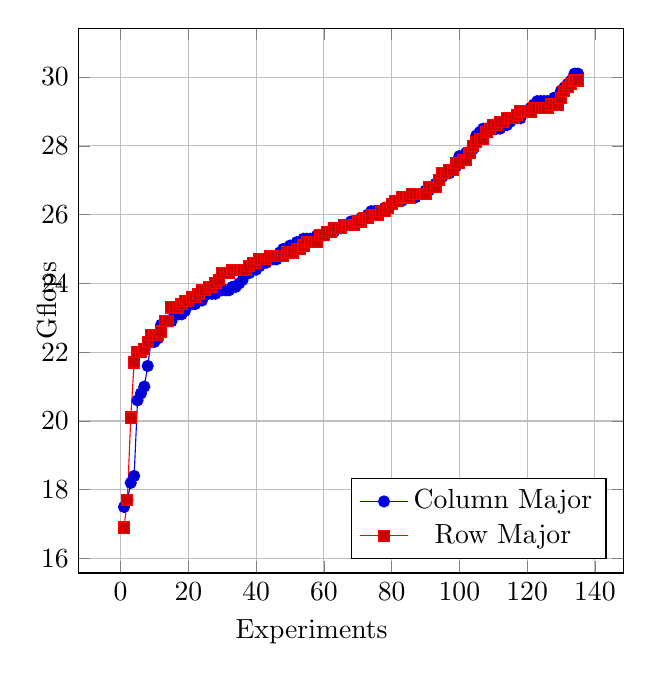
\begin{tikzpicture} 
	\begin{axis}[ 
        ylabel={Gflops},ylabel style={yshift=-0.5cm},
        xlabel={Experiments},xlabel style={xshift=-0.5cm},
		height=8.5cm, 
		width=8.5cm, 
		grid=major, 
		legend style={at={(0.5,0.1)},anchor=west},
	] 
	
	\addplot coordinates { 
	(1,1.75E+001)(2,1.77E+001)(3,1.82E+001)(4,1.84E+001)(5,2.06E+001)(6,2.08E+001)(7,2.10E+001)(8,2.16E+001)(9,2.23E+001)(10,2.23E+001)(11,2.24E+001)(12,2.28E+001)(13,2.29E+001)(14,2.29E+001)(15,2.29E+001)(16,2.31E+001)(17,2.31E+001)(18,2.31E+001)(19,2.32E+001)(20,2.34E+001)(21,2.34E+001)(22,2.34E+001)(23,2.35E+001)(24,2.35E+001)(25,2.37E+001)(26,2.37E+001)(27,2.37E+001)(28,2.37E+001)(29,2.38E+001)(30,2.38E+001)(31,2.38E+001)(32,2.38E+001)(33,2.39E+001)(34,2.39E+001)(35,2.40E+001)(36,2.41E+001)(37,2.43E+001)(38,2.43E+001)(39,2.44E+001)(40,2.44E+001)(41,2.45E+001)(42,2.46E+001)(43,2.46E+001)(44,2.47E+001)(45,2.47E+001)(46,2.47E+001)(47,2.49E+001)(48,2.50E+001)(49,2.50E+001)(50,2.51E+001)(51,2.51E+001)(52,2.52E+001)(53,2.52E+001)(54,2.53E+001)(55,2.53E+001)(56,2.53E+001)(57,2.53E+001)(58,2.54E+001)(59,2.54E+001)(60,2.54E+001)(61,2.55E+001)(62,2.55E+001)(63,2.55E+001)(64,2.56E+001)(65,2.56E+001)(66,2.57E+001)(67,2.57E+001)(68,2.58E+001)(69,2.58E+001)(70,2.58E+001)(71,2.59E+001)(72,2.59E+001)(73,2.60E+001)(74,2.61E+001)(75,2.61E+001)(76,2.61E+001)(77,2.61E+001)(78,2.62E+001)(79,2.62E+001)(80,2.63E+001)(81,2.64E+001)(82,2.64E+001)(83,2.64E+001)(84,2.65E+001)(85,2.65E+001)(86,2.65E+001)(87,2.65E+001)(88,2.66E+001)(89,2.66E+001)(90,2.67E+001)(91,2.67E+001)(92,2.68E+001)(93,2.69E+001)(94,2.70E+001)(95,2.71E+001)(96,2.72E+001)(97,2.72E+001)(98,2.73E+001)(99,2.74E+001)(100,2.77E+001)(101,2.77E+001)(102,2.78E+001)(103,2.78E+001)(104,2.79E+001)(105,2.83E+001)(106,2.84E+001)(107,2.85E+001)(108,2.85E+001)(109,2.85E+001)(110,2.85E+001)(111,2.85E+001)(112,2.85E+001)(113,2.86E+001)(114,2.86E+001)(115,2.87E+001)(116,2.88E+001)(117,2.88E+001)(118,2.88E+001)(119,2.90E+001)(120,2.90E+001)(121,2.91E+001)(122,2.92E+001)(123,2.93E+001)(124,2.93E+001)(125,2.93E+001)(126,2.93E+001)(127,2.93E+001)(128,2.94E+001)(129,2.94E+001)(130,2.96E+001)(131,2.97E+001)(132,2.98E+001)(133,2.99E+001)(134,3.01E+001)(135,3.01E+001)
	}; 
	\addlegendentry{Column Major} 
	
	\addplot coordinates { 
	(1,1.69E+001)(2,1.77E+001)(3,2.01E+001)(4,2.17E+001)(5,2.20E+001)(6,2.20E+001)(7,2.21E+001)(8,2.23E+001)(9,2.25E+001)(10,2.25E+001)(11,2.25E+001)(12,2.26E+001)(13,2.29E+001)(14,2.29E+001)(15,2.33E+001)(16,2.33E+001)(17,2.33E+001)(18,2.34E+001)(19,2.35E+001)(20,2.35E+001)(21,2.36E+001)(22,2.36E+001)(23,2.37E+001)(24,2.38E+001)(25,2.38E+001)(26,2.39E+001)(27,2.39E+001)(28,2.40E+001)(29,2.41E+001)(30,2.43E+001)(31,2.43E+001)(32,2.43E+001)(33,2.44E+001)(34,2.44E+001)(35,2.44E+001)(36,2.44E+001)(37,2.44E+001)(38,2.45E+001)(39,2.46E+001)(40,2.46E+001)(41,2.47E+001)(42,2.47E+001)(43,2.47E+001)(44,2.48E+001)(45,2.48E+001)(46,2.48E+001)(47,2.48E+001)(48,2.48E+001)(49,2.49E+001)(50,2.49E+001)(51,2.49E+001)(52,2.50E+001)(53,2.50E+001)(54,2.51E+001)(55,2.52E+001)(56,2.52E+001)(57,2.52E+001)(58,2.52E+001)(59,2.54E+001)(60,2.54E+001)(61,2.55E+001)(62,2.55E+001)(63,2.56E+001)(64,2.56E+001)(65,2.56E+001)(66,2.57E+001)(67,2.57E+001)(68,2.57E+001)(69,2.57E+001)(70,2.58E+001)(71,2.58E+001)(72,2.59E+001)(73,2.59E+001)(74,2.60E+001)(75,2.60E+001)(76,2.60E+001)(77,2.61E+001)(78,2.61E+001)(79,2.62E+001)(80,2.63E+001)(81,2.64E+001)(82,2.64E+001)(83,2.65E+001)(84,2.65E+001)(85,2.65E+001)(86,2.66E+001)(87,2.66E+001)(88,2.66E+001)(89,2.66E+001)(90,2.66E+001)(91,2.68E+001)(92,2.68E+001)(93,2.68E+001)(94,2.70E+001)(95,2.72E+001)(96,2.72E+001)(97,2.73E+001)(98,2.73E+001)(99,2.75E+001)(100,2.75E+001)(101,2.76E+001)(102,2.76E+001)(103,2.78E+001)(104,2.80E+001)(105,2.81E+001)(106,2.82E+001)(107,2.82E+001)(108,2.84E+001)(109,2.85E+001)(110,2.86E+001)(111,2.86E+001)(112,2.87E+001)(113,2.87E+001)(114,2.88E+001)(115,2.88E+001)(116,2.88E+001)(117,2.89E+001)(118,2.90E+001)(119,2.90E+001)(120,2.90E+001)(121,2.90E+001)(122,2.91E+001)(123,2.91E+001)(124,2.91E+001)(125,2.91E+001)(126,2.91E+001)(127,2.92E+001)(128,2.92E+001)(129,2.92E+001)(130,2.94E+001)(131,2.96E+001)(132,2.97E+001)(133,2.98E+001)(134,2.99E+001)(135,2.99E+001)
	}; 
	\addlegendentry{Row Major} 
	
	\end{axis} 
\end{tikzpicture}
	\caption{Performance impact of process mapping}
	\label{fig:PMAP}
\end{figure}


% ====================
\section{Challenges}
\label{sec:challenges}
% ====================

Initially, it proved difficult to get HPL working on the development machines as the documentation for HPL is sparsely spread across the web and leaves room for improvement. After successful installation a installation script (see appending \ref{sec:appendix_installationScript}) was created to serve as guideline for future users. The availability and/or correct functionality of some libraries are system dependent, thus the script might have to adapted for other systems.

Another challenge was building HPL on SuperMUC since none of the authors have experience with this systems. In the process of migrating the laptop installation, several adjustments had to be made to adopt the system architecture, such as replacing ATLAS by Intel's MKL, using an Intel specific MPI implementation, as well as locating all required libraries and necessary arguments. At this point we would like to thank one of our supervisors Isa\'ias Compr\`es Ure\~na for his continuous support.

Unfortunately, at the time of completing the plugin for this project SuperMUC maintenance hindered us from retrieving the necessary data required for evaluation. Previously, the plugin was built and properly executed on SuperMUC. During test runs a performance of about 174 Gflops was measured, without any optimization applied. The plugin is expected to function properly once maintenance is over and necessary adaptions due to system changes were performed.

% ====================
\section{Conclusion}
\label{sec:conclusion}
% ====================

In the course of this project a Periscope plugin was created to automate tuning of the HPL benchmark. Results show that it correctly points to the best scenario of all executed experiments. Brute forcing over all possible parameter combinations guarantees finding the optimal solution, but the execution time is unfeasibly long. Therefore a smarter approach should be applied to limit the search domain (see section \ref{sec:futureWork}). The plugin also supports optimization by execution time measured by Periscope and HPL with few adaptations. Evaluation of a large scale HPC system should to be performed in order to show the full capabilities of our plugin.

% ====================
\section{Future Work}
\label{sec:futureWork}
% ====================

Currently the plugin tries to brute force an optimal solution by trying every possible configuration. As this process is very expensive concerning computation time for the allocated resources, an intelligent approach to limit the search space should be applied in addition to common sense. For example the 270 experiments mentioned in this paper took several hours to complete. One might improve the search techniques and utilize online manipulation of benchmark parameters based on the latest benchmark results. Another approach is predicting the system performance by modeling it based on the system's architecture. By not applying brute force, the optimum solution might not be found as the risk of finding a local performance maximum exists.

In the course of this project "flops per second" was used as benchmark metric. Although widely used to classify supercomputers the resulting value can only serve as a baseline for comparison. In general, users of HPC systems desire a minimal execution time and/or low cost. For example "Tianhe-2" has a lower power to performance ratio than "Titan", second place in TOP500, which result in higher usage costs \cite{top500}. Thus, the fastest TOP500 system not necessarily yields the best results for every stakeholder. To optimize by execution time, the presented periscope plugin can be adapted to determine the average execution time over several runs and use it as benchmark metric. Likewise, the energy consumption of a system can be monitored using likwid-powermeter \cite{likwidLRZ,likwidPowermeter}.

Further, HPL solves dense matrix-matrix multiplication problems, but real-life HPC applications also contain differential equations, which need high bandwidth,low latency and irregular data access patterns, which HPL cannot execute efficiently. A new benchmark, called the High Performance Conjugate Gradient (HPCG) can deal better with lower computation-to-data-access ratios\cite{betterLinpack}. Moreover, LINPACK doesn't address issues like system latency and memory hierarchy. 

\begin{thebibliography}{9}
\raggedright
\bibitem{top500}
  	TOP500 Supercomputer Site,
  	\emph{November 2014}.
  	http://www.top500.org/lists/2014/11/
\bibitem{likwidLRZ}
	Leibnitz Supercomputing Centre,
	\emph{likwid - light weight performance tools}.
	https://www.lrz.de/services/software/program-mierung/likwid/
\bibitem{likwidPowermeter} 
	Liwkid,
	\emph{LikwidPowermeter}.
	https://code.google.com/p/likwid/wiki/Likwid-Powermeter
\bibitem{blas}
	BLAS,
	\emph{Basic Linear Algebra Subroutines}.
	http://www.netlib.org/blas/
\bibitem{atlas}
	ATLAS,
	\emph{Automatically Tuned Linear Algebra Software}.
	http://math-atlas.sourceforge.net/
\bibitem{HPLtuning}
	HPL,
	\emph{HPL Tuning}.
	http://www.netlib.org/benchmark/hpl/ tuning.html
\bibitem{dongarraluszczek}
	Luszczek and A. Petitet,
	\emph{The LINPACK Benchmark: Past, Present and Future},
	2001, University of Tennessee, USA
\bibitem{HPLexplained}
	Netlib,
	\emph{HPL Algorithm}.
	http://www.netlib.org/benchmark/hpl\_oldest/ algorithm.html
\bibitem{betterLinpack}
	Jack Dongarra and Michael Michael Heroux,
	\emph{Toward a new metric for ranking high performance computing systems},
	Sandia Report, SAND2013-4744, Volume 312, 2013
\bibitem{tibidabo}
	Tibidabo,
	\emph{Making the case for an ARM-based HPC system},
	Future Generation Computer Systems, Elsevier, 2013
\bibitem{apsc}
	Miceli, Civario, Sikora, César, Gerndt, Haitof, Navarrete, Benkner, Sandrieser, Morin, and Bodin,
	\emph{AutoTune: A Plugin-Driven Approach to the Automatic Tuning of Parallel Applications}, Lecture Notes in Computer Science, p. 328-342, 2013, Springer Berlin Heidelberg, Germany
\bibitem{mpitut}
	Blaise Barney,
	\emph{Message Passing Interface (MPI)},
	Lawrence Livermore National Laboratory.
	https://computing.llnl.gov/tutorials/mpi/
\bibitem{ompi}
	The Open MPI Project,
	\emph{A High Performance Message Passing Library}, 2015.
	http://www.open-mpi.org/
\bibitem{flow}
	Periscope,
	\emph{Periscope Tuning Framework Tutorials: Tuning Plugin Interface}.
	http://periscope.in.tum.de/releases/latest/ doxygen/a00004.html
\end{thebibliography}

\begin{appendices}
\onecolumn
\section{Installation Script}
\label{sec:appendix_installationScript}

\begin{lstlisting}
#!/usr/bin/env bash
cd ~


### PERISCOPE ###

# install dependencies
apt-get install -y bison flex build-essential gfortran libace-dev libxerces-c-dev libboost-all-dev doxygen automake autoconf libtool m4 libswitch-perl git mpich2
# clone repo
git clone http://periscope.in.tum.de/git-releases/PTF-PPE-Lecture.git
# prepare build
cd PTF-PPE-Lecture
./bootstrap
cd .. 
mkdir build 
cd build
# configure
../PTF-PPE-Lecture/configure --prefix=$HOME/install/periscope --enable-developer-mode 
# find out number of cores
NP=`cat /proc/cpuinfo | grep processor | wc -l`
# build framework
make -j $NP
make install
export PATH=$HOME/install/periscope/bin:$PATH
echo "export PATH=$HOME/install/periscope/bin:$PATH" >> ~/.bashrc


### BLAS ###

# For more information see following resources:
# http://linuxtoolkit.blogspot.de/2013/03/running-linpack-hpl-test-on-linux.html 

mkdir -p ~/src/
cd ~/src/
wget http://www.netlib.org/blas/blas.tgz
tar -zxvf blas.tgz
cd BLAS
gfortran -O3 -std=legacy -m64 -fno-second-underscore -fPIC -c *.f
ar r libfblas.a *.o
ranlib libfblas.a
rm -rf *.o
export BLAS=~/src/BLAS/libfblas.a
ln -s libfblas.a libblas.a
mv ~/src/BLAS /usr/local/


### ATLAS ###

# For more information see following resources:
# http://math-atlas.sourceforge.net/atlas_install/node6.html

cd ~
# disbale cpu throtteling
# Note: CPU throtteling might not be neccessary for virtual machines
apt-get install -y gnome-applets
apt-get install -y gnome-applets-data
#UNABLE TO LOCATE PACKAGE# apt-get install -y libpanel-applets2-0
/usr/bin/cpufreq-selector -g performance &

# download latest ATLAS library
wget http://www.netlib.org/lapack/lapack-3.5.0.tgz
wget http://sourceforge.net/projects/math-atlas/files/Stable/3.10.2/atlas3.10.2.tar.bz2
tar -xvf atlas3.10.2.tar.bz2
mv ATLAS ATLAS3.10.x                          # get unique dir name
cd ATLAS3.10.x                                # enter SRCdir
mkdir Linux_C2D64SSE3                         # create BLDdir
cd Linux_C2D64SSE3                            # enter BLDdir

../configure -b 64 --shared --with-netlib-lapack-tarfile=/home/$USER/lapack-3.5.0.tgz
# Note: These next steps might take very long...
make build                                    # tune & build lib
make check                                    # sanity check correct answer
make ptcheck                                  # sanity check parallel
make time                                     # check if lib is fast
make install                                  # copy libs to install dir


### OpenMPI ###

# For more information see following resources:
# http://www.sysads.co.uk/2014/05/install-open-mpi-1-8-ubuntu-14-04-13-10/

cd ~
# download latest package
wget https://www.open-mpi.org/software/ompi/v1.8/downloads/openmpi-1.8.4.tar.gz
apt-get install -y libibnetdisc-dev
tar -xvf openmpi-1.8.4.tar.gz
cd openmpi-1.8.4.tar.gz
./configure --prefix="/home/$USER/.openmpi"
make
make install
export PATH=$HOME/.openmpi/bin:$PATH
echo "PATH=$HOME/.openmpi/bin:$PATH" >> ~/.bashrc
export LD_LIBRARY_PATH=$HOME/.openmpi/lib/:$LD_LIBRARY_PATH
echo "LD_LIBRARY_PATH=$HOME/.openmpi/lib/:$LD_LIBRARY_PATH" >> ~/.bashrc


### HPL ###

cd ~
# download latest package
wget http://www.netlib.org/benchmark/hpl/hpl.tgz
tar -xvf hpl.tgz
cd hpl
# configure
ARCH="Linux_PII_CBLAS"
cp setup/Make.$ARCH .

# change parameters and practice sed
sed -i '/^ARCH*/ c\ ARCH = $(ARCH)' Make.$ARCH
sed -i '/^TOPdir*/ c\ TOPdir = $(HOME)/hpl' Make.$ARCH
sed -i '/^MPdir*/ c\ MPdir = /usr/lib/openmpi' Make.$ARCH
sed -i '/^MPinc*/ c\ MPinc = -I$(MPdir)/include' Make.$ARCH
sed -i '/^MPlib*/ c\ MPlib = $(MPdir)/lib/libmpi.so' Make.$ARCH
sed -i '/^LAdir*/ c\ LAdir = /usr/local/atlas/lib' Make.$ARCH
sed -i '/^CC*/ c\ CC = /usr/bin/mpicc' Make.$ARCH
sed -i '/^LINKER*/ c\ LINKER = /usr/bin/mpicc' Make.$ARCH

make arch=$ARCH
cd bin/$ARCH

# run HPL
mpirun -np 4 ./xhpl
\end{lstlisting}

\newpage
\section{HPL.dat for Laptop}
\label{sec:appendixHPLdatLaptop}
\begin{lstlisting}
HPLinpack benchmark input file
Innovative Computing Laboratory, University of Tennessee
HPL230.out   output file name (if any)
6            device out (6=stdout,7=stderr,file)
1            # of problems sizes (N)
10000        # N -- fantastically important; see ahead
1            # Number of block sizes
160          # Block sizes
1            PMAP process mapping (0=Row-,1=Column-major)
1            # of process grids (P x Q)
2            # Ps
2            # Qs
16.0         threshold
1            # of panel fact<
0            PFACTs (0=left, 1=Crout, 2=Right)
1            # of recursive stopping criterium
4            NBMINs (>= 1)
1            # of panels in recursion
2            NDIVs
1            # of recursive panel fact.
1            RFACTs (0=left, 1=Crout, 2=Right)
1            # of broadcast
3            BCASTs (0=1rg,1=1rM,2=2rg,3=2rM,4=Lng,5=LnM)
1            # of lookahead depth
1            DEPTHs (>=0)
2            SWAP (0=bin-exch,1=long,2=mix)
64           swapping threshold
0            L1 in (0=transposed,1=no-transposed) form
0            U in (0=transposed,1=no-transposed) form
1            Equilibration (0=no,1=yes)
8            memory alignment in double (> 0)
\end{lstlisting}

\end{appendices}

\end{document}